\section{Setup}
\label{sec:setup}
\begin{figure*}[htb!]
\centering
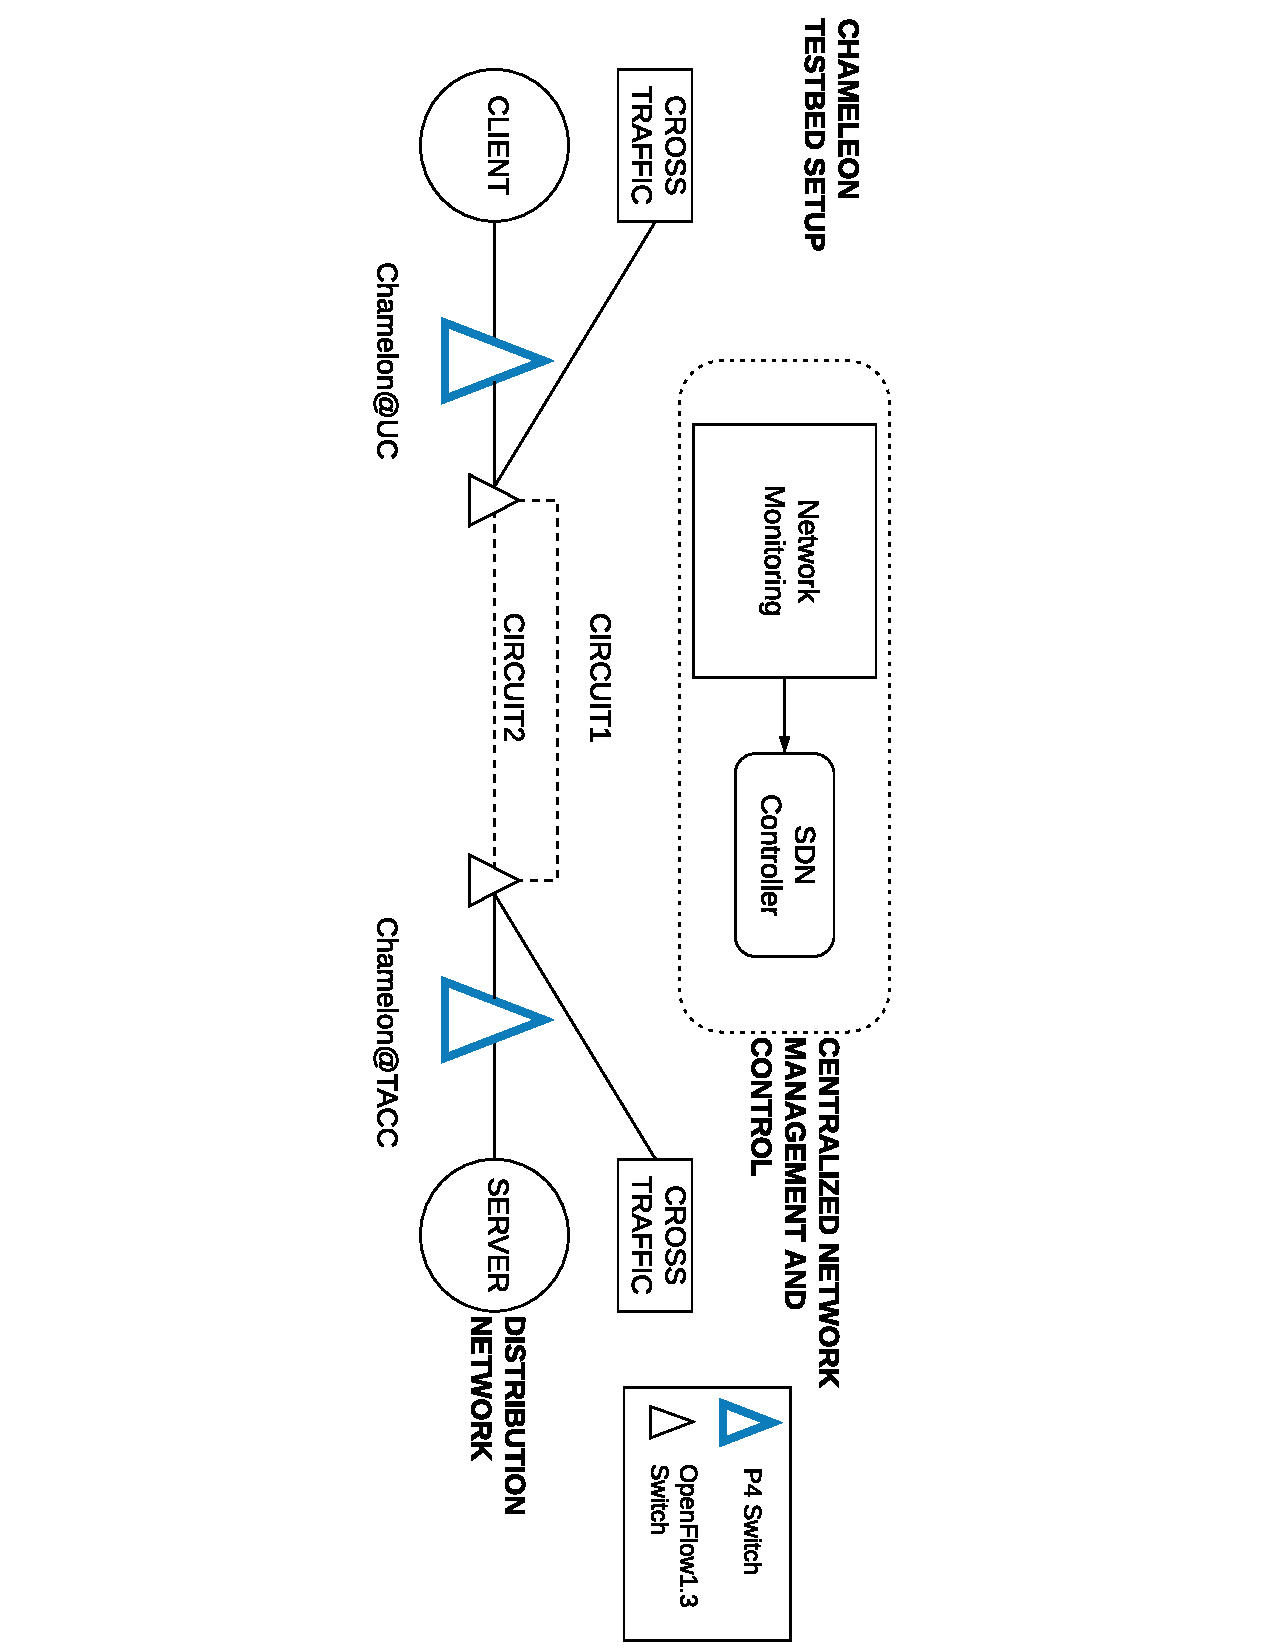
\includegraphics[width=.23\textwidth,trim={6cm 6cm 5cm 6cm}, angle=90] {figures/CHAMELEON_Exp.pdf}
\caption{Chameleon Testbed Setup: A HTTP/2 based video streaming client uses two disjoint paths to request multiple qualities of the same segment.}
\label{fig:p4-testbed}
\vspace{-14pt}
\end{figure*}
\subsection{Chameleon Testbed}
The Chameleon testbed is a deeply reconfigurable testbed that is suitable for large-scale prototyping of distributed systems and software defined networks. In this work, we leverage the recently released Bring-Your-Own-Controller feature along with previously existing capabilities of the Chameleon Cloud to create a prototype of our architecture. Figure \ref{fig:p4-testbed} shows the setup of our testbed, which we describe in detail.
\subsubsection{HTTP/2 application}
For the HTTP/2 application we instantiate two bare-metal nodes: one that emulates a Web server using the open source \texttt{Caddy} (version=0.10.10) software and another that emulates an ABR video streaming client, \texttt{AStream}{\footnote{\url{https://github.com/pari685/AStream}}}, that we modify to use an open-source Python-based library, \texttt{hyper}\footnote{\url{https://github.com/Lukasa/hyper}}, that downloads video content using HTTP/2. Note that the cross traffic nodes are bare-metal machines used to create various network congestion scenarios using \texttt{Iperf3}\footnote{\url{https://iperf.fr/iperf-download.php}} for controlled experiments.
\subsubsection{P4 Switch\cite{Bosshart:2014}}
We install the behavioral model, \texttt{BMV2}\footnote{\url{https://github.com/p4lang/behavioral-model}}, software switch components in a bare-metal node, which emulates a P4-capable switch, and then use the \texttt{P4Runtime}\footnote{\url{https://github.com/p4lang/PI}} tool to programmatically install rules into each switch. In future, we plan to replace this with a hardware ASIC P4 switch\footnote{\url{https://www.barefootnetworks.com/products/brief-tofino/}} that has only recently become available. 
\subsubsection{OpenFlow Switch}
OpenFlow \cite{McKeown:2008}, a widely-used implementation of SDN, is available to experimenters as a Virtual Forwarding Context (VFC), a functionality provided by Corsa switches, which enables each testbed user to provision a nearly-isolated instance of an OpenFlow (v1.3) switch. After HTTP/2 headers are translated into Q-in-Q tags as described in Sect. \ref{subsec:http2-header}, the application packets are forwarded through the Corsa switch into the core network.
\subsubsection{Core Network}
In this demonstration, we provision two VLAN circuits (denoted as \textit{Circuit1} and \textit{Circuit2}) between University of Chicago (UC) and Texas Advanced Computing Center (TACC) using the Advanced Layer-2 Service (AL2S) implemented by Internet2, which is a network service provider for collaborative research\footnote{\url{https://www.internet2.edu/products-services/advanced-networking/layer-2-services/#features-al2s}}.
\subsubsection{Centralized Management and Control}
For orchestration and visualization, we use Jupyter Notebooks \cite{kluyver2016jupyter}, an open-source web tool particularly suited for reproducible experiments. For this demonstration, Jupyter runs inside Chameleon and provides us with a single interface not only to run the controller and the ABR video streaming application but also to visualize network traffic and QoE metrics. 
 %We will provide a laptop that connects to the monitor and allows conference attendees to view as well as use the Jupyter web instance to interact with our experiment. 



